\documentclass[11pt]{article}

\usepackage{fullpage,times}%charter}
\usepackage{color}

\usepackage{tikz}
\usetikzlibrary{arrows.meta}

%% macros
\newcommand{\ax}[1]{\texttt{AX}(#1)}
\newcommand{\ex}[1]{\texttt{EX}(#1)}
\newcommand{\af}[1]{\texttt{AF}(#1)}
\newcommand{\ef}[1]{\texttt{EF}(#1)}
\newcommand{\ag}[1]{\texttt{AG}(#1)}
\newcommand{\eg}[1]{\texttt{EG}(#1)}
\newcommand{\au}[2]{\texttt{A}(#1\ \texttt{U}\ #2)}
\newcommand{\eu}[2]{\texttt{E}(#1\ \texttt{U}\ #2)}
\newcommand{\sem}[1]{[\!\![#1]\!\!]}

\newcommand{\sol}[1]{{\color{blue}#1}}

\begin{document}

\hrule
\smallskip

\noindent
\emph{Please review and study the solutions for homework assignment 1
before proceeding with this assignment. }

\noindent
You can review the latex source for this assignment-file to
learn and use latex to prepare your homework submission. You will see
the use of macros (to write uniformly formatted text), different
text-styles (emphasized, bold-font), different environments (figures,
enumerations).

It is not required that you use exactly this latex source to prepare
your submission. 
\smallskip
\hrule


\begin{center}
{\Large\bf Homework 2 (CTL): ComS/CprE/SE 412, ComS 512}

\medskip

Due-date: Feb 17 at 11:59PM.

\medskip


\end{center}

\noindent
\textbf{
Submit online on Canvas two files: the source file in latex format and
the pdf file generated from latex. Name your files:
$\langle\mbox{your-net-id}\rangle$-hw2.$\langle\mbox{tex/pdf}\rangle$.
}

\hrule
\noindent
\smallskip

\emph{ Homework must be individual's original work. Collaborations and
  discussions of any form with any students or other faculty members
  or soliciting solutions on online forums are not allowed. Please
  review the academic dishonesty policy on our syllabus. If you have
  any questions/doubts/concerns, post your questions/doubts/concerns
  on Piazza and ask TA/Instructor.}

\smallskip
\hrule

\begin{enumerate}

\item
Consider the following Kripke structure, with $p\in L(s_0) \cap L(s_2)$ and
$q\in L(s_2)$.
\begin{center}
    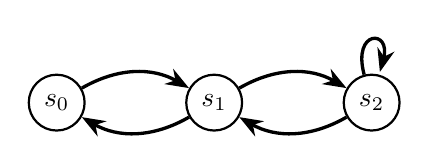
\begin{tikzpicture}
\begin{scope}[every node/.style={circle,thick,draw}]
    \node (s0) at (0,0) {$s_0$};
    \node (s1) at (2,0) {$s_1$};
    \node (s2) at (4,0) {$s_2$};
\end{scope}

\begin{scope}[>={Stealth[black]},
              every node/.style={fill=white,circle},
              every edge/.style={draw=black,very thick}]
    \path [->] (s0) edge[bend left=30] (s1);
    \path [->] (s1) edge[bend left=30] (s0);
    \path [->] (s1) edge[bend left=30] (s2);
    \path [->] (s2) edge[bend left=30] (s1);
    \path [->] (s2) edge[loop above] (s2);
\end{scope}
\end{tikzpicture}
\end{center}
Identify the set of states that satisfy each of the following and justify your answer:
\begin{enumerate}
\item $\ag{p} =\{ \}$
\item $\af{p}= \{s_0, s_1, s_2\}$
\item $\ag{\af{p}} = \{s_0, s_1, s_2\}$
\item $\af{\ag{p}} = \{ \}$  
\end{enumerate}
\hfill(2+2+3+3 pts)

\item Express the following statements as CTL formula:
\begin{enumerate}

\item
  There exists an execution sequence such that from every configuration in the sequence,
  it is possible to eventually satisfy the property $p$.
  
\textbf{Answer}: $\eg{\ef{p}}$
\item
  Along all paths, whenever $p$ is true, it is followed by a state where $p$ is false, and
  whenever $p$ is false, it is followed by a state where $p$ is true.
  
\textbf{Answer}:  $\ag{(p\rightarrow \ax{\neg p}) \land (\neg p \rightarrow \ax{p})}$
\end{enumerate}
\hfill (4+4 pts)

\item Prove or disprove the following:
  \begin{enumerate}
  \item
    If a state satisfies $\af{\ag{p}}$ then along all paths from that state the property $p$
    holds infinitely often.

    \textbf{Answer}: Let's assume, $$s_0 \in [[\af{\ag{p}}]]$$

    $$ \Rightarrow \forall \pi \in Path(s_0). \exists i \geq 0. \pi(i) \in [[\ag{p}]]$$
    $$ \Rightarrow \forall \pi \in Path(s_0). \exists i \geq 0. \forall \pi^\prime \in Path(\pi(i)).\forall j >=i.\pi^\prime(j) \in [[p]] $$


    
   This simplification tells that in all evaluations starting from the initial state, there exists a state from where $p$ holds in all paths globally. Due to the property of $\af$, $\ag$ might be satisfied at the very initial state, therefore, we can write the following if it is satisfied in the initial state.  

   $$ \Rightarrow \forall \pi \in Path(s_0).\forall j >=0.\pi(j) \in [[p]]$$
   
   
   However, the question asks whether this CTL formula satisfies $p$
    holds infinitely often. Since $p$ holds globally in all paths, $\af{\ag{p}}$ disproves the property $p$
    holds infinitely often. 

    The following Kripke structure satisfies $\af{\ag{p}}$ but it does not satisfies that the property $p$ holds infinitely often.


    
  \begin{center}
  \begin{tabular}{cc}
  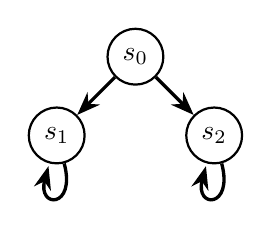
\begin{tikzpicture}
\begin{scope}[every node/.style={circle,thick,draw}]
    \node (s0) at (0,0) {$s_0$};
    \node (s1) at (-1,-1) {$s_1$};
    \node (s2) at (1,-1) {$s_2$};
\end{scope}

\begin{scope}[>={Stealth[black]},
              every node/.style={fill=white,circle},
              every edge/.style={draw=black,very thick}]
    \path [->] (s0) edge (s1);
    \path [->] (s0) edge  (s2);
    \path [->] (s1) edge[loop below] (s1);
    \path [->] (s2) edge[loop below] (s2);
\end{scope}
  \end{tikzpicture}
  &
  %%
  \begin{tabular}{l}
    $L(s_0) = \{p\}$ $L(s_1) = \{p\}$, $L(s_2) = \{p\}$
    \end{tabular}
  \end{tabular}
\end{center}

    \item
    If a state satisfies $\af{\ag{p}}$ then along all paths from that state the property $\neg p$
    holds finitely many times. 
            
\textbf{Answer}: It is immediate from question $3.a$ that, $\af{\ag{p}}$ does not guarantee to hold $\neg p$ finitely many times, because the value of $i$ might be anything greater than or equal to 0. If $i$ becomes 0,  $\ag{p}$ holds in the initial state. Therefore, $\af{\ag{p}}$ does not ensure $\neg p$ holds finitely many times. The Kripke structure provided in the same question also corroborates that the property $\neg p$ does not hold finitely many times. 

  \item  If a state satisfies $\eg{\ef{p}}$ then there exists at least one path starting from that
    state where $p$ holds infinitely often.
    
\textbf{Answer}:

If a state satisfies $\eg{\ef{p}}$, it does not necessarily true that $p$ holds infinitely often. Consider the following Kripke structure-

  \begin{center}
  \begin{tabular}{cc}
  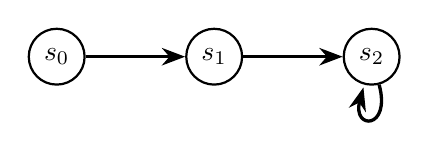
\begin{tikzpicture}
\begin{scope}[every node/.style={circle,thick,draw}]
    \node (s0) at (0,0) {$s_0$};
    \node (s1) at (2,0) {$s_1$};
    \node (s2) at (4,0) {$s_2$};
\end{scope}

\begin{scope}[>={Stealth[black]},
              every node/.style={fill=white,circle},
              every edge/.style={draw=black,very thick}]
    \path [->] (s0) edge (s1);
    \path [->] (s1) edge (s2);
    \path [->] (s2) edge[loop below] (s2);
\end{scope}
  \end{tikzpicture}
  &
  %%
  \begin{tabular}{l}
    $L(s_0) = L(s_2)= \{\}$, $L(s_1) = \{p\}$
    \end{tabular}
  \end{tabular}
\end{center}

This Kripke structure satisfies $\eg{\ef{p}}$ at $s_0$, but it does not satisfy $p$ to be true infinitely often in this path. 

% Let's assume, $$s_0 \in [[\eg{\ef{p}}]]$$

% $$ \Rightarrow \exists \pi \in Path(s_0). \forall i \geq 0. \pi(i) \in [[\ef{p} ]]$$
% $$\Rightarrow \exists \pi \in Path(s_0) \forall i \geq 0. \pi(i) [ \exists \pi^\prime \in Path(\pi(i)). \exists j \geq i.\pi^\prime(j) \in [[p]]]$$
% This implies that there exists at least one path that satisfies $p$ infinitely often. So, this statement holds. 
  
  \item $\au{p}{\ax{q}}$ is equivalent to $p \land \ax{\au{p}{q}}$

  \textbf{Answer}: Let's simplify  $\au{p}{\ax{q}}$ and $p \land \ax{\au{p}{q}}$ first. 

  We know $\au{\varphi}{\psi}$ can be written as $\psi \lor (\varphi \land \ax{\au{\varphi}{\psi}})$. So, we can write, 
  $$\au{p}{\ax{q}} \Leftrightarrow \ax{q} \lor (p \land \ax{\au{p}{\ax{q}}})$$

  
  We can claim a state $s$ satisfies $\au{p}{\ax{q}}$ if it satisfies either $\ax{q}$ or $p \land \ax{\au{p}{\ax{q}}}$. 
  


    Similarly, $$p \land \ax{\au{p}{q}} \Leftrightarrow p \land \ax{q \lor (p \land \ax{\au{p}{q}})}$$


Now, let's construct the following Kripke structure satisfying $\au{p}{\ax{q}}$. 


  \begin{center}
  \begin{tabular}{cc}
  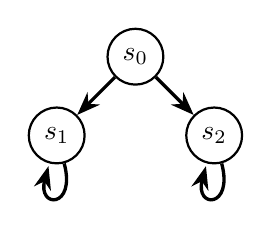
\begin{tikzpicture}
\begin{scope}[every node/.style={circle,thick,draw}]
    \node (s0) at (0,0) {$s_0$};
    \node (s1) at (-1,-1) {$s_1$};
    \node (s2) at (1,-1) {$s_2$};
\end{scope}

\begin{scope}[>={Stealth[black]},
              every node/.style={fill=white,circle},
              every edge/.style={draw=black,very thick}]
    \path [->] (s0) edge (s1);
    \path [->] (s0) edge  (s2);
    \path [->] (s1) edge[loop below] (s1);
    \path [->] (s2) edge[loop below] (s2);
\end{scope}
  \end{tikzpicture}
  &
  %%
  \begin{tabular}{l}
    $L(s_0)=\{\}, L(s_1) = \{q\}$, $L(s_2) = \{q\}$
    \end{tabular}
  \end{tabular}
\end{center}

From the above simplification, we know the above Kripke structure satisfies $\au{p}{\ax{q}}$ because it holds $\ax{q}$. However, it does not satisfy $p \land \ax{\au{p}{q}}$ because it requires $p$ to be true at the initial state.  
  
Therefore, we can say that $\au{p}{\ax{q}}$ is not equivalent to $p \land \ax{\au{p}{q}}$.

    
  \item \emph{For 512. Extra credit for 412 students}
    The property, \emph{for all paths of the form $\pi$, $p$ is true in every $\pi[i]$ where $i$ is even},
    can be expressed in CTL.
    
     \textbf{Answer}: 
    

    This question did not explicitly say about the odd position. Therefore, there are two cases to consider in the odd position. 
    Odd position may either hold $p$ or $ \neg p$. Even if the odd position holds any of $p$ or $\neg p$, it does not have an impact on the even position. 

    Let's consider a path, $\pi = s_0, s_1, s_2, ..., s_n, s_{n+1}, ... s_{n+k}, ...$. Considering $p$ holds in the even and odd position, we get the trace of the paths, $trace(\pi)= \{p, p, p, p, p, p, ... \}$, which we can represent as $\ag{p}$. Again, considering $\neg p$ holds in the odd position, we get the trace, $trace(\pi) = \{p, \neg p, p, \neg p, p, \neg p, ... \}$, which can be represented as $\ag{\af{p}}$. 

    Now the question is- does this formula enough to represent $p$ to be true in the even position? What if the trace becomes $trace(\pi) = \{\neg p, p, \neg p, p, \neg p, p, ... \}$. We can also represent this path using $\ag{\af{p}}$. However, these CTL formulas cannot restrict the path to hold $p$ in the even position. Therefore, we cannot write a CTL formula that can represent a path that satisfies $p$ to be true in the even position. 

    
  \end{enumerate}
  \hfill (2+2+3+3+4 pts)
  
\end{enumerate}


\end{document}

